\documentclass{article}
\usepackage[danish]{babel}
\usepackage{graphicx}
\usepackage{outlines}
\usepackage{amssymb}
\usepackage{enumitem}
\usepackage{listings}
\usepackage{tabularx}
\usepackage{multirow}
\usepackage{listings}
\usepackage[T1]{fontenc}
\usepackage{inconsolata}
\usepackage{color}
\usepackage{hyperref}
\renewcommand{\labelitemi}{$\bullet$}
\renewcommand{\labelitemii}{$\circ$}
\renewcommand{\labelitemiii}{$\blacksquare$}
\renewcommand{\labelitemiv}{$\star$}
\definecolor{pblue}{rgb}{0.13,0.13,1}
\definecolor{pgreen}{rgb}{0,0.5,0}
\definecolor{pred}{rgb}{0.9,0,0}
\definecolor{pgrey}{rgb}{0.46,0.45,0.48}
\lstset{language=Java,
  showspaces=false,
  showtabs=false,
  breaklines=true,
  showstringspaces=false,
  breakatwhitespace=true,
  commentstyle=\color{pgreen},
  keywordstyle=\color{pblue},
  stringstyle=\color{pred},
  basicstyle=\ttfamily,
  moredelim=[il][\textcolor{pgrey}]{$$},
  moredelim=[is][\textcolor{pgrey}]{\%\%}{\%\%}
}
\title{Bachelor thesis template}
\author{Claus Kramath}
\begin{document}
\maketitle
\thispagestyle{empty}
\newpage
\tableofcontents
\thispagestyle{empty} 
\newpage
\section{Introduktion}
\paragraph{}
I denne artikel skal vi se på de danske tegn; æ, ø samt å. Samtidig skal vi beskæftige os med deres større pendanter; Æ, Ø og Å.
\subparagraph{}
Vi skal ligeledes se på grafik i form af billeder. De kan både skaleres og sidestilles. Samtidig kan de refereres vha. labels, så sidetal og figur refereres automatisk og korrekt.
\subparagraph{}
Bemærk iøvrigt, at denne introduktion er skrevet med paragraph og subparagraph.
\newpage
\section{Grafik}
    \begin{figure}[h!]
        \begin{center}            
            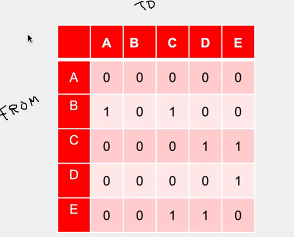
\includegraphics[scale=1.0]{images/picture.png}            
            \caption{Social network connections}
            \label{fig:1}
        \end{center}
    \end{figure}
    \begin{figure}[h!]
        \begin{center}
            \caption{See figure below}
            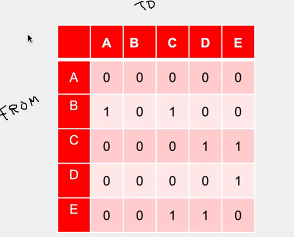
\includegraphics[scale=.5]{images/picture.png}
        \end{center}
    \end{figure}
    \begin{figure}[htb!]
        \begin{minipage}[t]{.5\textwidth}
            \centering
            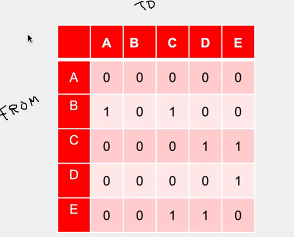
\includegraphics[scale=1]{images/picture.png}            
        \end{minipage}
        \begin{minipage}[t]{.5\textwidth}
            \centering
            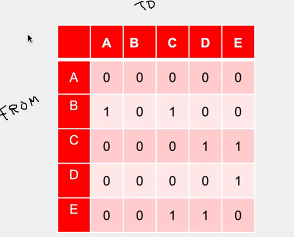
\includegraphics[scale=1]{images/picture.png}            
        \end{minipage}
        \caption{Two images side by side}
    \end{figure}
\newpage
\section{Referencer}
\paragraph{}
Vi skal se på hvordan vi refererer til en figur med en label.
    \subsection{Billeder}        
    \paragraph{}
        Som det kan ses af figur \ref{fig:1} er social networking spændende. Billedet viser hvilke personer (A-E) der er forbundet med hinanden.
        \subsubsection{Sider}
        \paragraph{}
        Billedet findes på side \pageref{fig:1}. Vha. billedets label kan vi automatisk finde frem til det korrekte sidetal.
\section{Unummererede sektioner}
\paragraph{}
I det følgende demonstreres, hvordan unummererede sektioner ser ud i \LaTeX:
\subsection*{Unummereret subsection}
\paragraph{}
    Her må der ikke være nummerering.
\subsubsection*{Unummereret subsubsection}
\paragraph{}
    Her må der heller ikke være nummerering.
\section{Lister}
\paragraph{}
Vi skal se på lister, som både kan ordnes nummerisk (ordnede) eller med bullet points (uordnede). Vi starter med de nummeriske og bevæger os siden over i lister med bullet points.
\subsection{Ordnede lister}
\paragraph{} 
Her først en nummererede lister, bemærk at listen har en indlejret, ordnet liste:

\begin{enumerate}
    \item Velkomst
    \item Første punkt på dagsordenen
    \item Næste punkt på dagsordenen
    \item Eventuelt, herunder:
    \begin{enumerate}
        \item Spørgsmål fra salen
        \item Glemte sager
        \item Forslag
    \end{enumerate}
\end{enumerate}
\paragraph{}
Nu skal vi se en kombination, dvs. en ordnet liste med en indlejret, uordnet liste:
\begin{enumerate}
    \item Velkomst
    \item Første punkt på dagsordenen
    \item Næste punkt på dagsordenen
    \item Eventuelt, herunder:
    \begin{itemize}
        \item Spørgsmål fra salen
        \item Glemte sager
        \item Forslag
    \end{itemize}
\end{enumerate}
\subsection{Uordnede lister}
\paragraph{}
Nu skal vi se på de lister der vises med bullet points. Også de kan kombineres med indlejrede lister, her først med en ordnet liste:
\begin{itemize}
    \item Velkomst
    \item Introduktion til lister
    \item Nøjere gennemgang:
    \begin{enumerate}
        \item Ordnede lister
        \item Uordnede lister
        \item Indlejrede lister
    \end{enumerate}
\end{itemize}
\paragraph{}
Herunder kombineres 2 uordnede lister:
\begin{itemize}
    \item Velkomst
    \item Introduktion til lister
    \item Nøjere gennemgang:
    \begin{itemize}
        \item Ordnede lister
        \item Uordnede lister
        \item Indlejrede lister
    \end{itemize}
\end{itemize}
\paragraph{}
Til slut skal vi se på lister i flere dybder, dvs. med flere indlejrede lister under sig. Bemærk at det kræver pakken amssymb, som inkluderes i toppen af dokumentets kildekode således:
\begin{verbatim}
    \usepackage{amssymb}
\end{verbatim} 
Samtidig kan man definere niveauer og bullets vha. renewcommand:
\begin{verbatim}
    \renewcommand{\labelitemi}{$\bullet$}
    \renewcommand{\labelitemii}{$\circ$}
    \renewcommand{\labelitemiii}{$\blacksquare$}
    \renewcommand{\labelitemiv}{$\star$}
\end{verbatim}
\begin{itemize}
    \item Første niveau
    \begin{itemize}
        \item Andet niveau
        \begin{itemize}
            \item Tredie niveau
            \begin{itemize}
                \item Fjerde niveau
            \end{itemize}
        \end{itemize}
    \end{itemize}
\end{itemize}
\paragraph{}
Herunder ses en ordnet liste, hvor der i første niveau bruges romertal. Dette fordrer include af package 'enumitem'.
\begin{enumerate}[label=\Roman*]
    \item Første niveau
    \begin{enumerate}
        \item Andet niveau
        \begin{enumerate}
            \item Tredie niveau
            \begin{enumerate}
                \item Fjerde niveau
            \end{enumerate}
        \end{enumerate}
    \end{enumerate}
    \item Første niveau
\end{enumerate}
\section{Tabeller}
\paragraph{}
I det følgende skal vi se, hvordan tabeller bruges og tekst i celler formatteres korrekt.
\subsection{Tabeller}
\subsubsection{Simpel tabel med label}
\paragraph{}
Her ses en centreret, simpel tabel med 3x3 celler:
\begin{center}
\begin{tabular}{ c c c }
    cell1 & cell2 & cell3 \\
    cell4 & cell5 & cell6 \\
    celle 7 & celle 8 & sidste celle
\end{tabular}
\end{center}
\subsubsection{Tabel med tekstjustering}
\paragraph{}
Her har vi en tabel hvor teksten i venstre kolonne er venstrestillet og modsat i højre kolonne, bemærk at her har vi gjort brug af flg. pakke: 
\begin{verbatim}
    \usepackage{tabularx}\end{verbatim}
\paragraph{}
Læg også mærke til at cellerne er lige store.
\begin{center}
    \begin{tabularx}{0.6\textwidth} { 
        | >{\raggedright\arraybackslash}X 
        | >{\centering\arraybackslash}X 
        | >{\raggedleft\arraybackslash}X | }
       \hline
       ø.venstre & ø.midt & ø.højre \\
       \hline
       n.venstre  & n.midt  & n.højre  \\
      \hline
      \end{tabularx}
\end{center}
\subsubsection{Tabel med celler med colspan og rowspan}
\paragraph{}
Nedenfor ses en tabel med celler, som breder sig over hhv. flere kolonner og rækker. For at undgå at den horisontale linie går gennem cellen som spænder over flere rækker, kan man gøre flg.:
\begin{verbatim}
    \cline{2-6}
\end{verbatim}

\begin{center}    
    \begin{tabular}{|p{1.5cm}|c|c|c|c|c|}
        \hline
        \multirow{2}{*}{\parbox{1.5cm}{Cells 1 \& 7}}
        & cell 2 & \multicolumn{2}{|c|}{Cells 3 \& 4} & \multicolumn{2}{|c|}{Cells 5 \& 6} \\
        \cline{2-6}
        & cell 8 & cell 9 & cell 10 & cell 11 & cell 12 \\
        \hline
    \end{tabular}
\end{center}
\subsubsection{Tabel med labels og referencer}
\paragraph{}
For at en tabel kan have en label, skal den erklæres således:
\begin{verbatim}
    \begin{table}
        \begin{tabular}
            ...
        \end{tabular}
        \caption{tekst under tabellen} <-- dette nummererer også tabellen.
        \label{table:1} <-- refereres med \ref{table:1}
    \end{table}
\end{verbatim}
\paragraph{}
Her ses tabellen \ref{table:1} som har en label, der kan refereres:
\begin{table}[h!]
    \centering
    \begin{tabular}{ c c c }
        cell1 & cell2 & cell3 \\
        cell4 & cell5 & cell6 \\
        celle 7 & celle 8 & sidste celle
    \end{tabular}
    \caption{Her er tabellen som refereres i teksten.}
    \label{table:1}
\end{table}
\newpage
\section{Code listing}
\paragraph{}
I \LaTeX er det muligt at vise kode med syntax highlighting, så man nemmere kan se, hvad der foregår i koden. I eksemplet er der gjort brug af Java, men det er muligt at benytte mange andre sprog, blot det konfigureres korrekt.
\subsection{\LaTeX eksempel}
\paragraph{}
\LaTeX kode understøttes direkte ved at bruge:
\begin{lstlisting}[escapechar=+]
    +\verb!\begin{verbatim}!+
        ...
    +\verb!\end{verbatim}!+
\end{lstlisting}
\subsection{Java eksempel}
\begin{lstlisting}
    /**
     * This is a doc comment.
     */
    package com.ociweb.jnb.lombok;
    
    import java.util.Date;
    import lombok.Data;
    import lombok.EqualsAndHashCode;
    import lombok.NonNull;
    
    $$@Data
    $$@EqualsAndHashCode(exclude={"address","city","state","zip"})
    public class Person {
        enum Gender { Male, Female }
    
        // another comment
    
        %%@NonNull%% private String firstName;
        %%@NonNull%% private String lastName;
        %%@NonNull%% private final Gender gender;
        %%@NonNull%% private final Date dateOfBirth;
    
        private String ssn;
        private String address;
        private String city;
        private String state;
        private String zip;
    }
    \end{lstlisting}
\section{Matematiske udtryk}
\section{Bibliografi}
\section{Todo}
\paragraph{}
Her er først og fremmest en samling links, som der er benyttet til udarbejdelsen af denne skabelon.
\subsection{Links}
\href{https://www.overleaf.com/learn/latex/Code_listing}
\href{https://stackoverflow.com/questions/3019774/how-write-this-in-verbatim-latex}
\href{https://www.overleaf.com/learn/latex/Tables}
\end{document}
